\documentclass[11pt]{amsart}
\usepackage{geometry}                % See geometry.pdf to learn the layout options. There are lots.
\geometry{letterpaper}                   % ... or a4paper or a5paper or ... 
%\geometry{landscape}                % Activate for for rotated page geometry
%\usepackage[parfill]{parskip}    % Activate to begin paragraphs with an empty line rather than an indent
\usepackage{graphicx}
\usepackage{amssymb}
\usepackage{epstopdf}
\usepackage{caption}
\usepackage{subcaption}
\DeclareGraphicsRule{.tif}{png}{.png}{`convert #1 `dirname #1`/`basename #1 .tif`.png}

% Declare commands
\newcommand{\mat}[1]{\mathbf{#1}}

\title{CS 181 -- Practical 1}
\author{Casey Grun, Sam Kim, Rhed Shi}
%\date{}                                           % Activate to display a given date or no date

\begin{document}
\maketitle

\section{Warmup}
We used the K-Means algorithm to cluster the images of the CIFAR-10 dataset, which consists of 60000 total 32x32 color images. We only clustered a single batch, consisting of 10000 images. The algorithm was run for $k=5,10,15$.\\
The following sets of images show the mean images of the k clusters for $k=5,10,15$ as well as the 25 images that are closest to each of the respective means for $k=5,10$.\\

\begin{figure}[h]
	\centering
	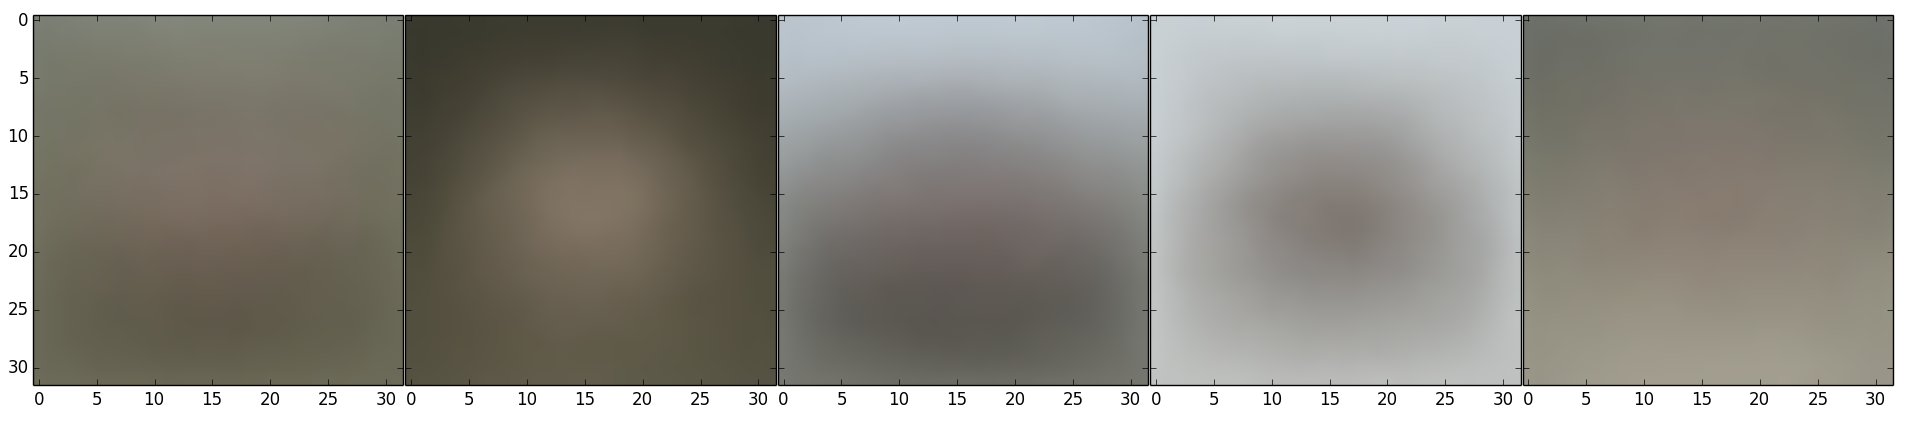
\includegraphics[width=8cm]{images/k5us.png}\\
	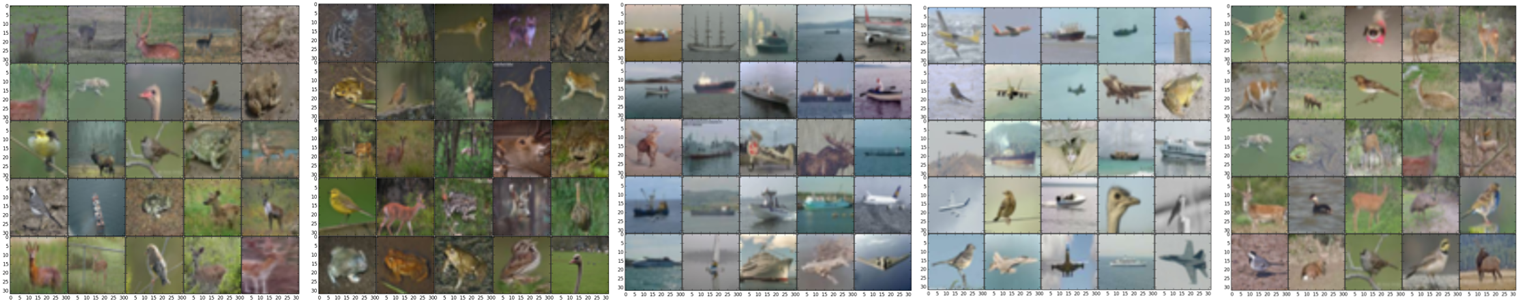
\includegraphics[width=15cm]{images/k5reps.png}\\
	\caption{(Top) Cluster means and (bottom) 25 representative images for each of the cluster means for $k=5$.}
\end{figure}

\begin{figure}[h]
	\centering
	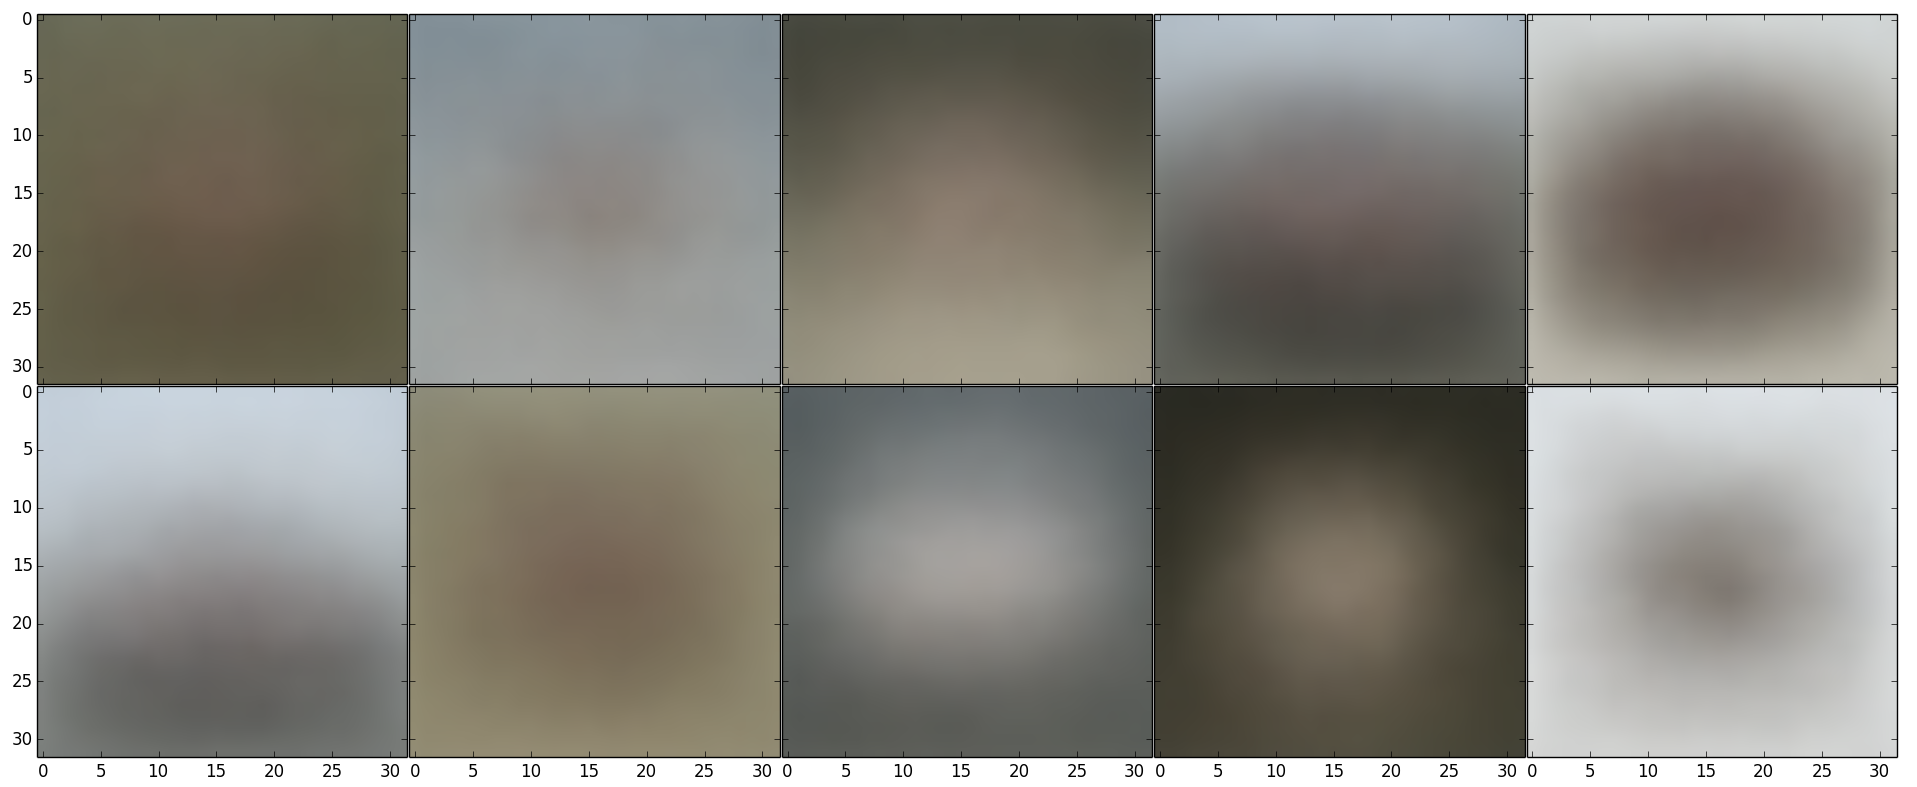
\includegraphics[width=8cm]{images/k10us.png}\\
	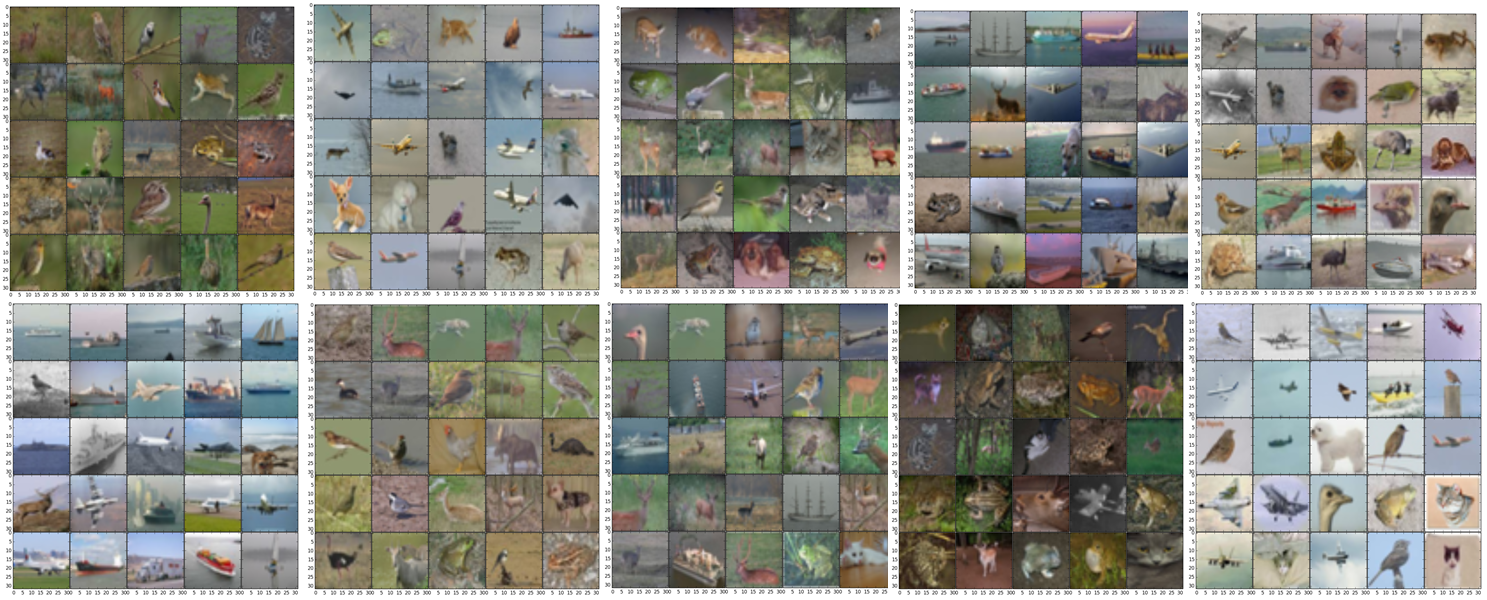
\includegraphics[width=15cm]{images/k10reps.png}\\
	\caption{(Top) Cluster means and (bottom) 25 representative images for each of the cluster means for $k=10$.}
\end{figure}

\begin{figure}
\centering
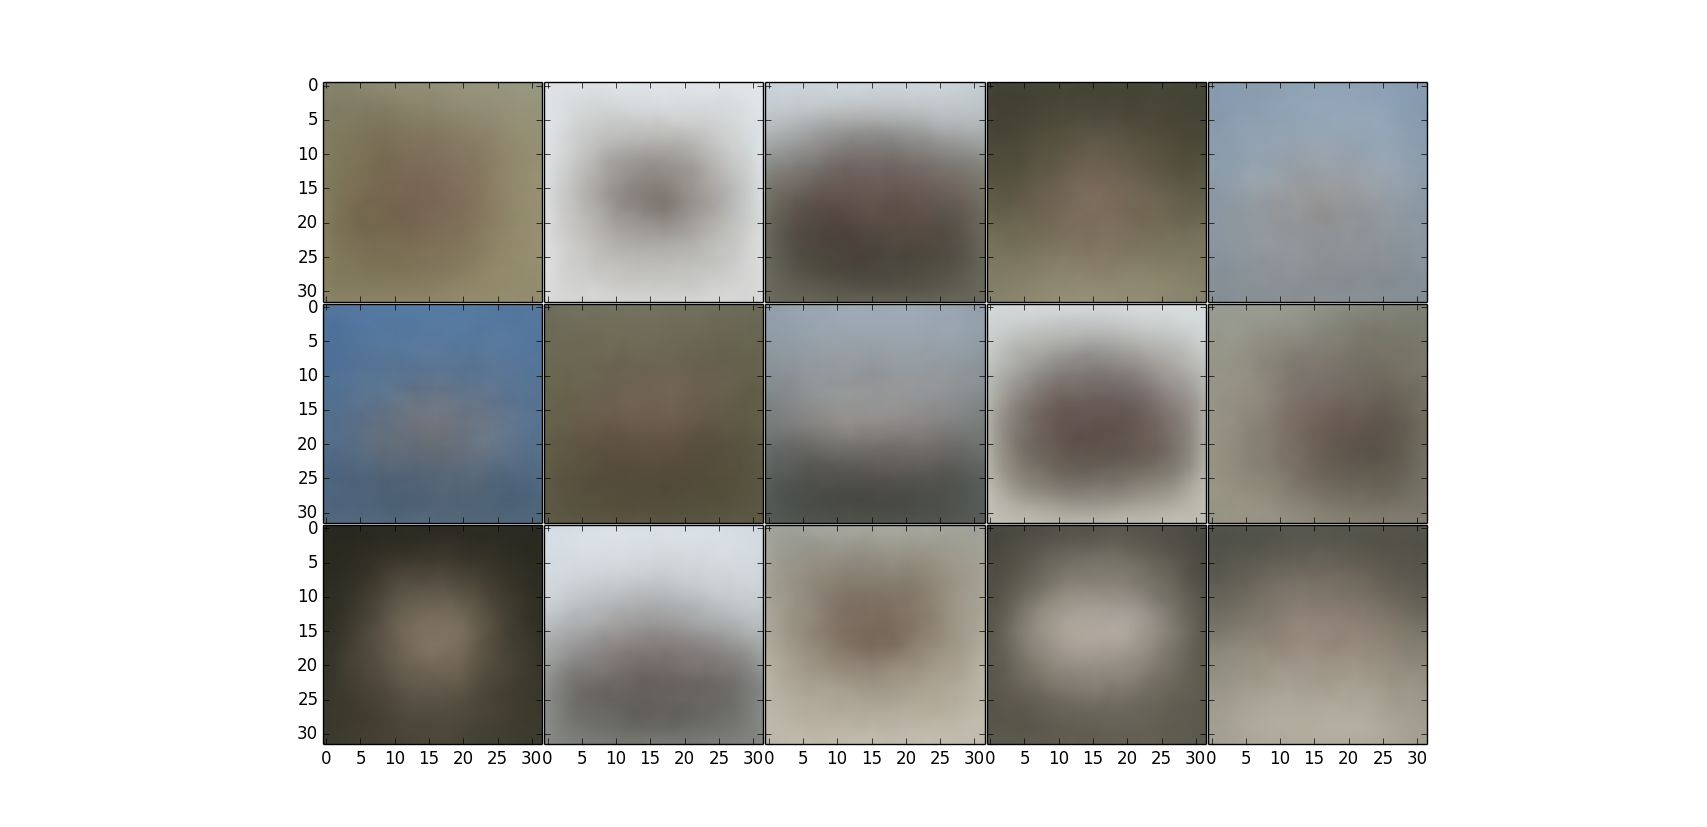
\includegraphics[width=7cm]{images/k15us.png}
\caption{Cluster means for $k=15$}
\end{figure}

Although features are not discernible from the mean images, there are still trends of lighter colors versus darker colors, which is consistent with the representative images. For example, in $k=5$, the 2nd cluster mean is mostly dark around the edges whereas the 4th cluster mean is mostly light around the edges, and the representative images share these features. Additionally, we see that as we increase $k$, the distinction between mean images increase as well. For $k=5$, the means are mostly greyish brown images, whereas for $k=15$, several of the mean images have tints of blue.\\

We use the objective function:
$$J(\{r_n\}^N_{n=1},\{\mu_k\}^K_{k=1})=\sum^N_{n=1}\sum^K_{k=1}r_{nk}||x_n-\mu_k||^2_2$$
where $r_n$ is the responsibilities vector of the $n$th data point, $\mu_k$ is the mean of the $k$th cluster, and $x_n$ is the $n$th data point. Plots of the objective function as a function of iteration for $k=5,10,15$ are shown below.


\begin{figure}[h]
	\centering
	\begin{subfigure}{0.5\textwidth}
		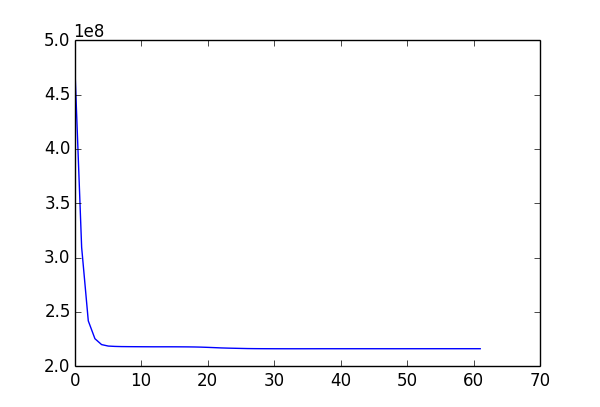
\includegraphics[width=7cm]{images/k5objectives.png}
		\caption{$k=5$}
	\end{subfigure}
	\begin{subfigure}{0.3\textwidth}
		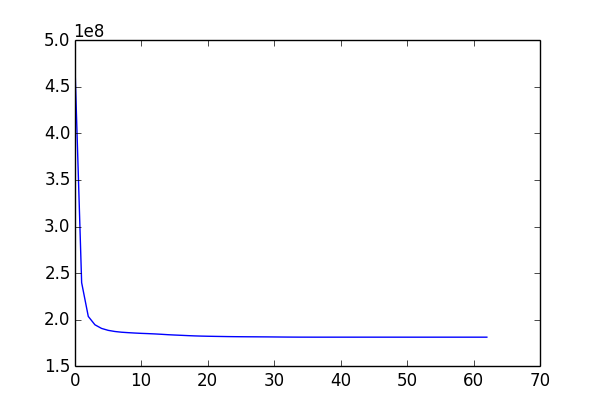
\includegraphics[width=7cm]{images/k10objectives.png}
		\caption{$k=10$}
	\end{subfigure}
	\begin{subfigure}{0.3\textwidth}
		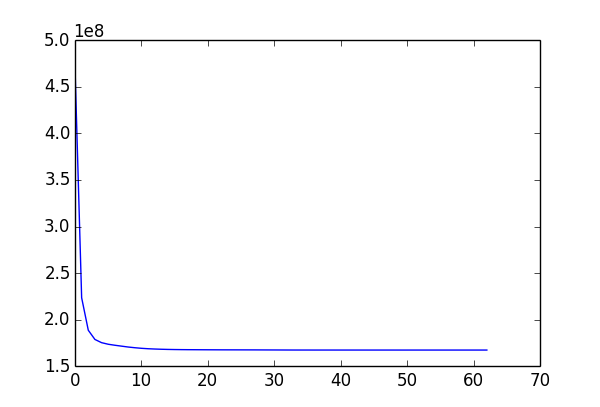
\includegraphics[width=7cm]{images/k15objectives.png}
		\caption{$k=15$}
	\end{subfigure}
	\caption{Objective function as a function of iteration for K-Means}
\end{figure}

We can see that for all 3 $k$s, the objective function never increases over the iteration, so the algorithm is constantly finding a better solution and converging to a (local) minimum. In addition, comparing the objective functions, $k=5$ reaches approximately $J=2.2\times 10^{8}$, $k=10$ converges to $J=1.8\times 10^{8}$, and $k=15$ converges to $J=1.7\times 10^{8}$. As suspected, allowing more clusters allows the images to be closer to their respective cluster means.\\

\begin{figure}[h]
	\centering
	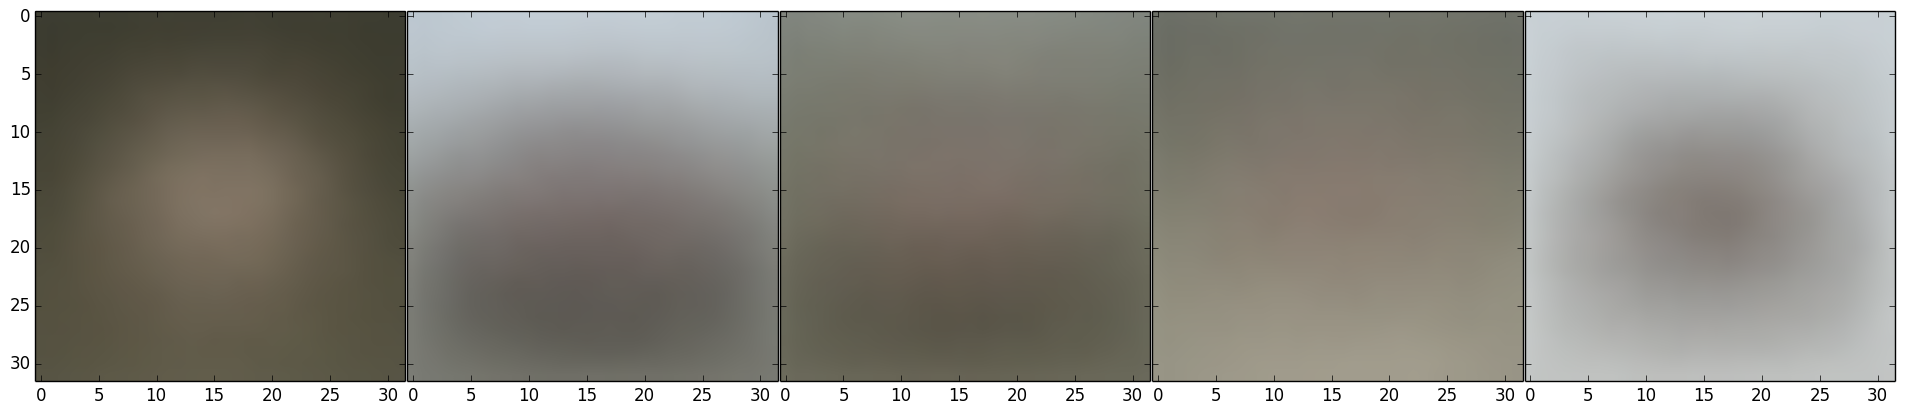
\includegraphics[width=8cm]{images/kplus5us.png}\\
	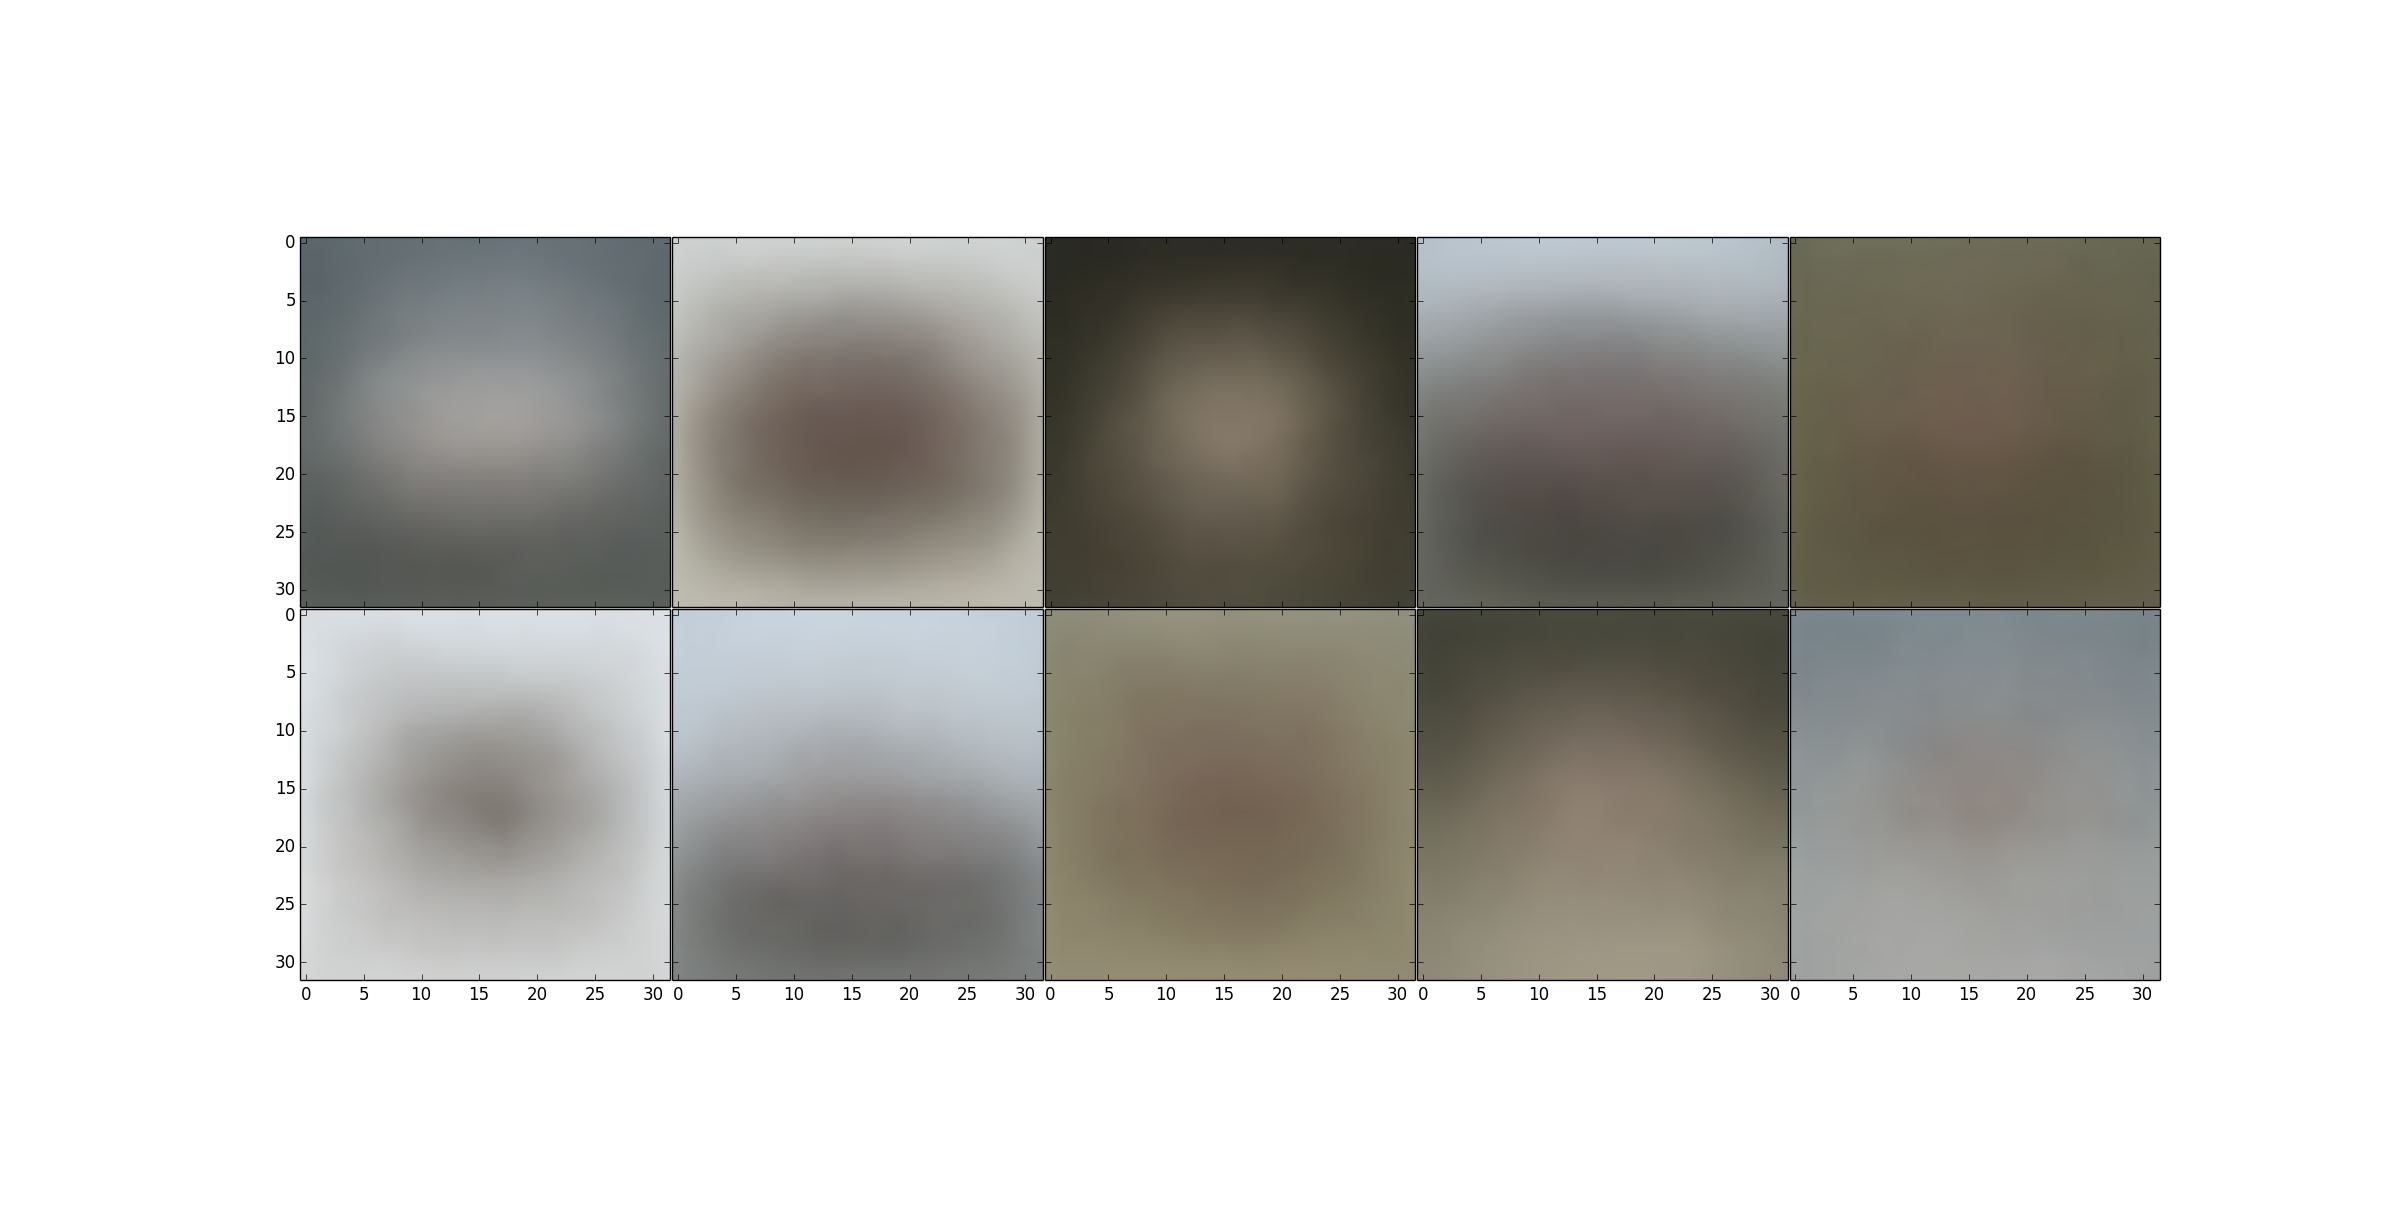
\includegraphics[width=8cm]{images/kplus10us.png}\\
	\caption{Cluster means for (top) $k=5$ and (bottom) $k=10$}
\end{figure}

We also implemented the K-Means++ algorithm. Shown below are mean images of the k clusters fo $k=5,10$. These are not qualitatively different from those of the K-Means algorithm. The objective function for $k=5$ reaches $J=2.15\times 10^{8}$, and for $k=10$ reaches $J=1.8\times 10^{8}$.

\section{Approaches considered}
K-Means, K-nearest neighbor, PCA, SVD, PMF

\section{Probabilistic Matrix Factorization}
\subsection{Derivation}
The probabilistic matrix factorization (PMF) approach \cite{Mnih:2007wg} attempts to decompose the ratings matrix $\mat{R}$ into two matrices: $\mat{P}$ representing the users and $\mat{Q}$ representing the books:
$$\mat{R} = \mat{P} \times \mat{Q}^T$$
where:
$$ 
\mat{P} = 
\begin{pmatrix}
	\vec{p_1} \\
	\vec{p_2} \\
	\vdots    \\
	\vec{p_N} 
\end{pmatrix} = 
\begin{pmatrix}
	p_{1,1} & p_{1,2} & \ldots & p_{1,K} \\
	p_{2,1} & p_{2,2} & \ldots & p_{2,K} \\
	\vdots  & \vdots  & \ddots & \vdots  \\
	p_{N,1} & p_{N,2} & \ldots & p_{N,K} \\
\end{pmatrix}
$$
$$ 
\mat{Q} = 
\begin{pmatrix}
	\vec{q_1} \\
	\vec{q_2} \\
	\vdots    \\
	\vec{q_N} 
\end{pmatrix} = 
\begin{pmatrix}
	q_{1,1} & q_{1,2} & \ldots & q_{1,K} \\
	q_{2,1} & q_{2,2} & \ldots & q_{2,K} \\
	\vdots  & \vdots  & \ddots & \vdots  \\
	q_{N,1} & q_{N,2} & \ldots & q_{N,K} \\
\end{pmatrix}
$$
Each entry $\vec{p_i}$ in $\mat{P}$ represents a vector of $K$ latent features of user $i$, while $\vec{q_j}$ represents the $k$ latent factors of the book. If we can produce the matrices $\mat{P}$ and $\mat{Q}$, we can predict any entry $r_{i,j}$ in $\mat{R}$ by taking inner products of the vectors $\vec{p_i}$ and $\vec{q_j}$:
$$\hat{r}_{i,j} = \vec{p_i} \cdot \vec{q_j}^T \approx r_{i,j}$$

However, we only know a subset of the full matrix $\{r_{i,j}\}_{i=1, j=1}^{N,D}$; call that subset $T = \{(i, j, r_{i,j})\}$. We therefore need to iteratively train $\mat{P}$ and $\mat{Q}$, based only on the data in $T$. 

We recognize that some aspects of the ratings for a particular book are not explained jointly by the user and book, but by either the user or the book alone; we follow the approach of Paterek, Koren and Bell, and others in calling these terms \emph{biases} \cite{Paterek:2007va,Koren:2009uc}. A bias is the component of a user's ratings (or a book's ratings) varying from the global mean, $\mu = \frac{1}{ND} \sum_{i=1}^{N}\sum_{j=1}^{D} r_{i,j}$. Let $\vec{b} = (b_1, b_2, \ldots b_N)$ represent the biases for each users and $\vec{c} = (c_1, c_2, \ldots c_D)$ represent the biases for each book. We will adopt a slightly more sophisticated model for predicting the ratings, such that:
$$\hat{r}_{i,j} = \mu + b_i + c_j + \vec{p_i} \cdot \vec{q_j}^T \approx r_{i,j}$$
or:
$$\mat{R} \approx \mat{P} \times \mat{Q}^T + (\mu + \vec{b} \otimes \vec{c})$$
where $\otimes$ is the outer product.

To learn the values of $\mat{P}$ and $\mat{Q}$, we will minimize an error function:
$$E = \sum_{i,j,r_{i,j} \in T} e_{i,j} $$
$$E = \sum_{i,j,r_{i,j} \in T} \left(r_{i,j} - \hat{r}_{i,j}\right)^2 + \frac{\beta}{2} \left( ||p_i||^2 + ||q_i||^2 + b_i^2 + b_j^2 \right) $$
The first term of this error function simply describes the squared reconstruction error. The second term enforces regularization---penalizing rows of $\mat{P}$ and $\mat{Q}$ that have high magnitude. 

From this expression, we can derive $\nabla e_{i,j}$; this will allow us to minimize $e_{i,j}$ (and hence $E$) by stochastic gradient descent.

\begin{align*}
\frac{\partial e_{i,j}}{\partial p_{i,k}} &= \frac{\partial}{\partial p_{i,k}} \left(r_{i,j} - \hat{r}_{i,j}\right)^2 + \frac{\partial}{\partial p_{i,k}} \frac{\beta}{2} \left( ||p_i||^2 + ||q_i||^2 + b_i^2 + b_j^2 \right) \\
    &= 2 \left(r_{i,j} - \hat{r}_{i,j}\right)  \left(-\frac{\partial}{\partial p_{i,k}} \hat{r}_{i,j}\right)  + \frac{\partial}{\partial p_{i,k}} \frac{\beta}{2} \left( ||p_i||^2\right) \\
    &= 2 \left(r_{i,j} - \hat{r}_{i,j}\right)  \left(-\frac{\partial}{\partial p_{i,k}} \left(\mu + b_i + c_j + \vec{p_i} \cdot \vec{q_j}^T \right) \right)  + \frac{\partial}{\partial p_{i,k}} \frac{\beta}{2} \left( ||p_i||^2 \right) \\
    &= 2 \left(r_{i,j} - \hat{r}_{i,j}\right)  \left(-\frac{\partial}{\partial p_{i,k}} \left( \sum_{k=1}^{K} p_{i,k} q_{j,k} \right) \right)  + \frac{\partial}{\partial p_{i,k}} \frac{\beta}{2} \left( \sum_{k=1}^{K} p_{i,k}^2 \right) \\
    &= -2 \left(r_{i,j} - \hat{r}_{i,j}\right)  \left(q_{j,k} \right) + \beta p_{i,k} \\
\frac{\partial e_{i,j}}{\partial q_{j,k}} &= -2 \left(r_{i,j} - \hat{r}_{i,j}\right)  \left(p_{i,k} \right) + \beta q_{j,k} \\
\frac{\partial e_{i,j}}{\partial b_{i}} &= -2 \left(r_{i,j} - \hat{r}_{i,j}\right) + \beta b_{i} \\
\frac{\partial e_{i,j}}{\partial c_{j}} &= -2 \left(r_{i,j} - \hat{r}_{i,j}\right) + \beta c_{j}
\end{align*}

We can therefore implement a set of update rules as follows:
\begin{align*}
p_{i,k} &\gets p_{i,k} + \alpha \left(2 \left(r_{i,j} - \hat{r}_{i,j}\right)  q_{j,k} - \beta p_{i,k} \right) \\
q_{j,k} &\gets p_{i,k} + \alpha \left(2 \left(r_{i,j} - \hat{r}_{i,j}\right)  p_{i,k} - \beta q_{j,k} \right) \\
b_{i}   &\gets p_{i,k} + \alpha \left(2 \left(r_{i,j} - \hat{r}_{i,j}\right)          + \beta b_{i}   \right) \\
c_{j}   &\gets p_{i,k} + \alpha \left(2 \left(r_{i,j} - \hat{r}_{i,j}\right)          + \beta c_{j}   \right)
\end{align*}

We update $\vec{p_i}$, $\vec{q_j}$, $b{i}$, and $c_{j}$ for each pair $(i, j, r_{i,j}) \in T$. This process is repeated for some number of steps, or \emph{epochs}, until either some criterion for epochs is met (e.g. the change in the total error $E$ is less than some $\epsilon$, or the maximum number of epochs is exceeded). 

\subsection{Optimization}
The main issue we had with the PMF approach was that there were lots of meta-parameters to tune: the learning rate $\alpha$, the regularization parameter $\beta$, the number of latent factors $K$, and the criteria for determining convergence. We estimated appropriate starting values for $K = 5$ and $\beta = 0.02$ based on literature on the Netflix prize \cite{Mnih:2007wg,Ott:2008tu}, and we experimented to determine that $\alpha = 0.001$ generally produced convergent solutions. We tried the following reductionist methods for validating our approach, and for further tuning these parameters:

\begin{enumerate}
\item Checking the gradient. We verified that our gradient function was correct by finite differences.
\item Recapitulating the user mean results. We tried setting $K=1$, $\beta=0$ and fixing $q_{j,k} = 1$. This gave us an RMSE of 0.77857---slightly better than the user mean results.
\item Reconstruction of fake data. We generated fake values for $\mat{P}$ and $\mat{Q}$, and multiplied them together to get a fake $\mat{R}$. We then trained the model on $T$ containing some fraction of the $r_{i,j}$'s.  
\item Cross-validation. We withheld a subset (between 1--10\%) of our training data, trained the model on the remainder, computed the difference between the predicted ratings and the withheld ratings. We used this method to attempt to set our parameters
 
\end{enumerate}

\subsection{Results and Conclusion}


\bibliography{library}
\bibliographystyle{ieeetr}


\end{document}  
